\documentclass[12pt]{book}
\usepackage{amsmath, amssymb, amsthm}
\usepackage{latexsym, epsfig, ulem, cancel, multicol, hyperref}
\usepackage{graphicx, tikz, subfigure,pgfplots}
\usepackage{blindtext}
\usepackage[a4paper, total={6in, 8in}]{geometry}
\setlength{\parindent}{0pt}
\usepackage{multirow}
\usepackage{mathtools}
\pgfplotsset{width=10cm,compat=1.9}

\title{\textbf{Theory of Relativity Notebook}}
\author{Dennis Li \thanks{Instructor: Prof. Gabriel Perez-Giz}}


\newcommand{\liminfty}[1]{\lim_{#1 \to \infty}}
\newcommand{\limzero}[1]{\lim_{#1 \to 0}}
\newcommand{\Z}{\mathbb{Z}}
\newcommand{\R}{\mathbb{R}}
\newcommand{\C}{\mathbb{C}}
\newcommand{\lineint}[1]{\int_{#1}}
\newcommand{\pypx}[2]{\frac{\partial #1}{\partial #2}}
\newcommand{\divg}{\nabla \cdot}
\newcommand{\curl}{\nabla \times}
\newcommand{\dydx}[2]{\frac{d #1}{d #2}}
\newcommand{\sqbkt}[1]{\left[ #1 \right]}
\newcommand{\paren}[1]{\left( #1 \right)}
\newcommand{\tribkt}[1]{\left< #1 \right>}
\newcommand{\abso}[1]{\left|#1 \right|}


\begin{document}

\maketitle
\tableofcontents

\part{Special Relativity}
\chapter{Spacetime - Taylor and Wheeler}
\section{Invariance of Spacetime Interval}

\subsection{Invariance of distance across methods of measurements}

Now let us consider a line segment in the xy-plane as follows
\begin{center}
\begin{tikzpicture}
\begin{axis}
\addplot[color=red]{x};
\end{axis}
\end{tikzpicture}
\end{center}
We can see that the line segment can be the hypotenuse of infinitely many right triangle, whole remaining the same length.\\
and this relationship satisfies the Pythagoras theorem:
\[
a^2+b^2=c^2
\]
Where $a$ and $b$ are the 2 sides of the right triangle, and $c$ is the hypotenuse.\\
Experimental results shows that there is a similar relationship between space and time.\\
Now we define a similar relationship, instead of on xy-plane, on a space-time plot, as shown below. 
\begin{center}
\begin{tikzpicture}
\begin{axis}[
xmin=-4,
xmax=4,
ymin=-4,
ymax=4,
axis lines=middle,
xlabel=distance,
ylabel=time,
]
\addplot[color=red,domain=-2:2]{x};
\end{axis}
\end{tikzpicture}
\end{center}
Here, we have a space-time plot. And the relationship is not Pythagorean. With experimental results, we find the this line segment follows a relationship such that
\[
\Delta s^2=-\Delta t^2 + \Delta r^2
\]
Where $\Delta s$ is the space-time interval and $\Delta t$ is the time interval, measured in meters, and $\Delta r$ is the spatial separation.\\
To make sense of this, we have to introduce more context.
\subsection{meters of time, event, spacetime interval}
Let us first get familiar with the concept of \textbf{Event.}\\\\
An \textbf{Event} is basically something that just happens, regardless of who is checking it out. An observer that is interested in a certain series of event (say, 2) could measure the following parameters. 
\begin{enumerate}
    \item The time separation between event 1 and event 2
    \item The spatial separation between event 1 and event 2
\end{enumerate}
One might be tempted to just use these measurements and tryout this relationship of spacetime interval, but there are more works to do before throwing in numbers. We would first have to unify the units of space and time such that the operation make sense.\\
\newline
We start with measuring time in meters, which is not conventional, yet familiar. As we often measures distance with time such as \textit{10 minutes away from school}. We would assume an underlying speed given the means of transportation. And for our purpose, the underlying speed is the speed of light $c$.\\
Therefore, the time we use for our practice would be 
\[
\Delta t = c\Delta t' 
\]
where $\Delta t'$ is time measured in seconds, and $c$ is the speed of light $(299792458\;m/s)$.\\
now we have a unit of time that is consistent with the measurement of spatial separation.\\
\\For example, $1ns$ or $1\times 10^{-9}s$ is $\approx 0.3$ \textit{meters of time}\\
\\A similar practice can be done for spatial separation if we are would like to have the units of distance comply with that of time.\\
\newline
For example, $1\; Au$ or \textit{1 astronomical unit} (The distance from the earth to the sun) is $499$ \textit{seconds of distance}. This means it takes light, the speed limit of the universe, $499$ seconds to cross this distance. 
\\
\\
The spacetime interval $\Delta s$ will have a unit corresponding to that of the choice for space and time.
\\\\
Note that, the spacetime interval may be negative in some cases, as long as we keep the minus sign consistent, it would resolve at the end of a calculation. But it is still preferably \textbf{kept positive}.\\
\\
Now that we are good with the units, let us talk about where did these intervals we are dealing with came from, where we have to introduce the concept of an \textbf{Spacetime interval}\\, one the other side of the equation.
\\
\newline
Just like the Pythagoras example we made earlier, there can be an indefinite amount of triangles that share the same hypotenuse. You can play around with the numbers of the sides of a right triangle while keeping the hypotenuse the same. We call this \textbf{Invariance of distance} across different methods of measurements. \\
\newline
This concept extends beyond spatial distance. With experimental data, we found that $\Delta s$, or the spacetime interval, is also invariance across different methods of measurement, or different observers. And this is a key concept that help us figure stuff out in the theory of relativity. \\
\newline
\textbf{Remark: }Note that there is a \textbf{minus sign} in the relationship between space and time, therefore it is not a straight forward relationship like a right triangle.

\subsection{Utilizing Invariance of spacetime interval}
After understanding the basics of this relationship, we can give some example of the utilization of this properties.\\
\newline
Assume there is a certain particle, say muon ($\mu$). It is currently traveling at a speed of $0.9c$ or 90\% the speed of light. The muon zips through 2 consecutive detectors installed in a laboratory. The 2 detectors are 1 meters apart. All the data was measured by observers in the laboratory. \\
\newline
We start by examining our events. Let muon crossing detector 1 be event 1, and the same for detector 2. We obtain the following data.
\[
\Delta t_{lab} = \frac{1}{0.9c} \;\;\; \Delta r_{lab} = 1m
\]
Now if we look at muon's perspective, something peculiar happens. \\
\newline 
If we look at muon's perspective, and treat it as \textit{stationary}, and the entire earth is zooming in front of it, we get some very different observations.\\
\\
First of which, the distance between event 1 and event 2 are $zero$. Since for the muon, both events happened right at his position. Therefore the relationship becomes the following
\[
\Delta t_\mu = \;? \;\;\; \Delta r_\mu = 0
\]
We noticed that something has changed. and if we remember that spacetime interval should stay constant across these 2 observers, we have achieved a way to figure out $\Delta t_\mu$.
\[
-\Delta t_\mu^2 = -\Delta t_{lab}^2 +\Delta r_{lab}^2
\]
simply multiply both side by $-1$ and divide the equation by $\Delta t_{lab}^2$, we get 
\[
\frac{\Delta t_\mu^2}{\Delta t_{lab}^2} = 1 - \frac{\Delta r_{lab}^2}{\Delta t_{lab}^2}
\]
we see that, for motion of no acceleration, $\frac{\Delta r_{lab}^2}{\Delta t_{lab}^2} = v$, it is the velocity, and it equals $0.9c$.
rewrite the equation, we have
\[
\frac{\Delta t_\mu^2}{\Delta t_{lab}^2} = 1-v^2
\]
\[
\Delta t_{lab}^2 = \frac{\Delta t_\mu^2}{1-v^2}
\]
\[
\Delta t_{lab} = \frac{\Delta t_\mu}{\sqrt{1-v^2}}
\]
since $v$ here is the ration of the object's speed and speed of light, we can redefine this parameter using Greek letter $\beta$
\[
\beta = \frac{v_o}{c}
\]
Now we have this relationship for the time separation for the muon:
\[
\Delta t_\mu = \gamma \Delta t_{lab} \;\;\; \gamma = \frac{1}{\sqrt{1-\beta^2}}
\]
\label{time dilation derivation}
If we carry out this calculation, we find that the time separation between the 2 events are greater than that of what we measured in the lab, it is as though that \textbf{time dilated} for muon. 

\section{Observer and frame of reference}

\subsection{Frame of Reference}
We start by imaging us free-falling from a rooftop wit an apple. If were to fall along with an enclosure that stops us from observing outside, we would think we are floating in the house without the influence of gravity. This is called a \textbf{free float} frame, or \textbf{free fall} frame.\\
\newline
Here, Newton's 1st law works just as one would expected. An object that is initially at rest relative to the frame remains at rest without force acted upon it. An object that is moving in a constant velocity wants to keep moving at the velocity. This is called \textbf{inertia}. And if Newton's 1st law so accurately describes such a free fall frame, we would call these \textbf{inertial frame}. 
\\
\newline
One may have noticed that there are discrepancies in this definition. The earth gravitational field is not uniform as it's magnitude decreases by inverse square law, and the direction vectors in 2 horizontally spaced position points towards the center of the earth instead of being parallel to each other. So if we are in a free fall frame that is big enough, or if we observe for a long enough time period, we would eventually spot the discrepancies and realize that we are inside a gravitational field. \\
\newline
This difference in gravity due to spatial separation is called an \textbf{tidal} effect. And owing to its existence, we have to refine our definition for inertial frame. \\
\newline
An Inertial frame would have to follow the following criteria:\\
\begin{enumerate}
    \item It has to obey Newton's 1st law.
    \item And only in this defined space and time, said frame of reference is inertial.
    \item Therefore, an inertial frame is \textbf{local}.
\end{enumerate}
Let us elaborate on the 3 criteria.\\
\newline
The definition of inertial reference frame rely on Newton's first law. We say a reference frame to be inertial if it obeys this law, which brings us to the second criteria.\\
\newline
Since gravity is not uniformly distributed in the space, there are bound to be inconsistencies with Newton's first law, or the law of inertia. Therefore we have to specify a certain time period and a limited size space to be our reference frame in which the inconsistencies with the law of inertia is not detectable or negligible in our desired precision. This can mean measuring precision or just a precision under which we deem insignificant. \\
\newline
With the first and second criteria explained, it is not hard to see why an inertial frame is local. We are working with very specific setup that we defined. And if we passes that specific setup, we can no longer treat the frame of reference inertial.\\
\newline
Also, we would call the object we are interested in observing a \textbf{test particle}. Such particle should experience the same acceleration across all none-unique inertial frame. This means, it would travel in a straight line in every inertial reference frame and for all observers in an inertial reference frame. And of course, \textit{same acceleration} is relative to the given measuring precision or desired precision. 

\subsection{Observers}
Now with the understanding of inertial frame, we can talk about observers.\\
\newline
An ideal observer in the special relativity setup can be imagined as a lattice of synchronized clocks that memorize where and when an event happened in an inertial frame. The conventional method for synchronizing such a lattice is using light pulse. We would set 1 clock to $00:00$, use it as a standard clock and set other clocks' time to $00:00+\Delta r$, where $\Delta r$ is distance ,measured in time, between each clock to the standard clock. Once the standard clock begin to record time, it sends a light pulse that, upon detection, activates other clocks. And now we have a lattice of synchronized clocks we can use to measure our data.\\
\newline
\textbf{Remark:} Setting up all the clocks at the same time and location and then bring them to the desired location would not work since their motion would inevitably dilates time, causing all the clocks to run a tiny slower. The severeness of this effect is related to how fast you move the clocks. 

\subsection{Summary}
We can now conclude this chapter with several important piece of information.
\begin{enumerate}
    \item \textbf{Inertial reference frame obey Newton's 1st Law of inertia}
    \item \textbf{Test particles experience the same acceleration in all inertial frame}
    \item \textbf{Inertial frame is only valid with given constraints on space and time}
    \item \textbf{Inertial frame is non-unique, choose whatever that makes calculation easy}
\end{enumerate}
If all 4 criteria are met, we can begin to study how particles, space, and time behave in inertial reference frames. And this study is called \textit{special relativity}. Special, since it has many limitations outside which it stops working. And the study that supports the study of space and time without this many limitations is \textbf{general relativity.}

\subsection{Some food for thoughts}
Let us show why defining a constraint in space and time is important for our study.\\
\newline
imagine there are 2 identical balls falling from 1 km. It would take them about ... W.I.P.

\section{Homogeneity of Inertial Reference Frames}
This chapter will focus on how the principle of relativity play a role in our study of special relativity.\\
\newline
The principle of relativity states that:
\begin{quote}
    \textit{All the laws of physics are the same in every free-float (inertial) reference frame.}
\end{quote}
\subsection{What is changed across inertial reference frame}
There are physical parameters that will change across inertial reference frame that are moving with a constant velocity relative to each other. And this section will discuss what would change in different inertial frame.\\
\newline
Time and distance is an obvious one since we have discussed it many times up to this point. But we can therefore derive more physical quantities that do not remain constant in different inertial frame. \\
\newline
If an object is moving relative to an observer that is at rest in his frame, then in the object's frame, it is stationary and the observer is moving relative to the object, this shows that velocity is not constant across frames. Another quantity that is not as obvious is acceleration. But if velocities is not the same across reference frame, so are acceleration. This implies that force is also not the same in different frame. And if this is true, then field would also not behave in the same way across different frame of reference. 
\subsection{What is the same across inertial reference frame}
In short, laws of physics stays the same in different frames. Even though forces, motions, or even energies may not be the same in different frames, the way they interact in a given frame always agree on the same universal law of physics. This comes from the negative version of the principle of relativity, stating that:
\begin{quote}
    \textit{No test of the laws of physics provides any way whatsoever to distinguish one free-float frame from another.}
\end{quote}
This means that there are no such thing as \textit{standard} frame, and any physical experiment would not yield a result that gives you a clue of whether you are moving at a constant velocity or at rest. \\
\newline
Therefore the physical constants that we are familiar with such as the permittivity of free space, permeability of free space, or gravitational constant would stay this same. Anything that is fundamental and cannot give you information on absolute motion would remain constant across frames. 
\subsection{Relativity of Simultaneity}
This one is a bit counter intuitive. An event that happens simultaneously in one frame cannot happen simultaneously in another frame that is moving relative to each other. \\
\newline 
Suppose a train moving on a railway got stroked by 2 lightnings at the front end and the rear end of the train simultaneously for observer that is at rest in his frame. For the observer on the moving train, these 2 event, however, did not happen on the same time. The lightning would strike the front end of the train first and then the rear end. 
\\
\newline
We can also think about this using the invariance of spacetime interval. If 2 events can happen simultaneously in 2 different frame, then we would have the following relationship:
\[
\Delta r_A^2 = \Delta r_B^2
\]
Experimental data showed that this is \textbf{not} a valid equality, which brings us to the next property in special relativity, \textbf{length contraction}.
\subsection{Length contraction}
Just like \textbf{time dilation}, length of an object is not invariant across inertial frames. With experimental data and calculation done with the invariant of spacetime interval, we find that for an observer that is at rest in his frame, an object that is moving would have its length contracted along the direction of its motion. However, the dimension that is transverse to the direction of its motion would be unchanged. \\
\newline
Such peculiar phenomenon is described as \textbf{Length Contraction}. We can see this relationship by thinking about the invariant of spacetime. \\
\newline
Suppose a set of experiment apparatus is situated in a moving train relative to an outside observer who is at rest in this frame. The apparatus is consisted of 2 fireworks that is situated \textbf{r} meters apart from each other. Now in the train, Alice set of both fireworks simultaneously in her frame, and the outside observer Bob recorded what he saw. We now have the following information.
\\
\newline

Derivation for length contraction goes in here.



\subsection{Summary}

summary here

\subsection{Practice}
\subsubsection{Derivation of relativistic speed addition}
First of all, we would imagine there to be a train moving with respect to an outside observer with speed $v_rel$ (as to relative velocity).

\section{Lorentz Transformation}
Lorentz transformation is a linear transformation that preserves the origin and the speed of light. It helps us to investigate how events across different references frame position themselves.
\subsection{Deriving the Lorentz transform}
Before going into deriving the Lorentz transform, we have to bear in mind several important requirements. First of all, the transformation have to preserve the invariant of spacetime interval. Secondly, the transformation must be linear; that is, an object going in a straight line with respect to one frame should also maintain a straight line motion after transformed. \\
\newline
Now we can start with the basic setup. Since the relativistic effects do not manifest on dimensions transverse to the direction of motion, we can confidently say that the coordinates would not change for the other 2 dimensions orthogonal to the direction of motion. We would denote them as $y$ and $z$, and $y'$, $z'$ in the transformed frame respectively. We have the following relationship:
\[
y=y' \;\;\; z=z'
\]
Now imagine a train traveling with respect to an observer that is rest at his frame. A spark plug flashes twice with certain time gap between it. Let's denote the first spark as $(0,0)$ on the spacetime diagram for both observer, and the second spark would be located at $t$ and $t'$ for the rest observer and the train observer. We can now express the $x$ coordinates of these 2 flashes as follows:
\[
x=\beta t
\]
where $\beta = \frac{v_{rel}}{c}$\\
\newline
Now we would like to figure out when and where in the train's reference frame do things happen. Since the first spark is coincidence in both frame and both spark happens at the same place for the train, we know that
\[
x=0 \;\; x'=0 \;\; \Delta x' = 0 \;\; \Delta t = t \;\; \Delta t' = t' \;\; \Delta x = \beta t
\]
Now let us consider the invariant spacetime interval
\[
t'^2=t^2-\beta t^2
\]
We have previously worked on this expression, we would obtain
\[
t=\gamma t'
\]
\[
\gamma \equiv \frac{1}{\sqrt{1-\beta ^2}}
\]
So we have obtained a relationship that works when events are coincident. But if we would like a more generalized transformation, we would have to consider the full relationship. The general form of this transformation can be considered in the following form
\[
t=Bx'+Dt'
\]
\[
x=Gx'+Ht'
\]
Or we can write this in a matrix form, since we are looking for a linear transformation
\[
\begin{bmatrix}
    t \\ x
\end{bmatrix}
=
\begin{bmatrix}
    D&B\\
    H&G
\end{bmatrix}
\begin{bmatrix}
    t'\\ x'
\end{bmatrix}
\]
Now we can start using our previous results to help with the derivation. 
\[
t = \gamma t' + Bx'
\]
\[
x=\gamma \beta t' + Gx' 
\]
The extra term of $x$ is to consider events that do not happen right on the origin. But we still let both frame share the same origin.\\
\newline
Based on the invariance of spacetime interval and the above underlying circumstances, we can obtain the following relationship
\[
t^2 - x^2 = t'^2 - x'^2
\]
plugging in the relationship we set up earlier
\[
(Bx'+\gamma t')^2 - (Gx' + \gamma \beta t')^2 = t'^2 - x'^2
\]
After expanding and regrouping, we obtain something like this
\[
\gamma^2(1-\beta^2)t'^2 +2\gamma(B-\beta G)x't' - (G^2 - B^2)x'^2 = t'^2 - x'^2
\]
we compare the left and right hand side of the equation, by the relationship of the coefficient between each term, we can deduce the following relationship
\[
\begin{cases}
    \gamma^2(1-\beta^2)=1\\
    2\gamma(B-\beta G)=0\\
    (G^2-B^2)=1
\end{cases}
\]
Here, we can obtain
\[
B=\beta G\\
\]
\[
G^2 - \beta ^2 G^2 = 1
\]
\[
G^2(1-\beta ^2 ) = 1
\]
\[
G = \gamma
\]
\[
\begin{cases}
    \gamma = \frac{1}{\sqrt{1-\beta^2}} \;\;\; \gamma \neq 0\\
    B=\beta G = \beta \gamma \\ 
    G = \gamma
\end{cases}
\]
We have figured out the entire lorentz transform.
\[
t = \gamma (t'+\beta x') \;\;\;
x = \gamma (x'+\beta t')
\]
And we can write it in the linear transformation form
\[
\begin{bmatrix}
    t \\ x
\end{bmatrix}
=
\begin{bmatrix}
    \gamma      &   \beta\gamma   \\
    \beta\gamma &   \gamma
\end{bmatrix}
\begin{bmatrix}
    t'\\ x'
\end{bmatrix}
\]
And the inverse transformation is just the inverse of the matrix, which can be easily obtained for a $M_{2 \times 2}$ matrix
\[
\begin{bmatrix}
    t' \\ x'
\end{bmatrix}
=
\begin{bmatrix}
    \gamma      &   -\beta\gamma   \\
    -\beta\gamma &   \gamma
\end{bmatrix}
\begin{bmatrix}
    t\\ x
\end{bmatrix}
\]
Or written explicitly
\[
t' = \gamma(t-\beta x)
\]
\[
x' = \gamma (x-\beta t)
\]
\subsection{Relativistic Speed Addition}
Since the speed of light is the absolute speed limit of the universe, we cannot surpass it. If you are on a train that is going in $0.9c$ relative to lab frame stationary on earth, you shoot a bullet that goes $0.9c$ relative to you, the bullet would certainly not travel $1.8c$ with respect to the earth. We have derived this once earlier using an explicit method.\\
\newline
But wit hthe newly acquired tool that is the Lorentz transformation, we can do it much more easily.\\
\newline
Let the lab frame be denoted by $t,x$, the train frame be $t',x'$, and the bullet frame be $t'', x''$. The speed of the bullect relative to the earth frame can simply be derived as the following
\[
\begin{bmatrix}
    t \\ x
\end{bmatrix}
=
\begin{bmatrix}
    \gamma      &   \beta\gamma   \\
    \beta\gamma &   \gamma
\end{bmatrix}
\begin{bmatrix}
    t'\\ x'
\end{bmatrix}
\]
\[
\begin{bmatrix}
    t' \\ x'
\end{bmatrix}
=
\begin{bmatrix}
    \gamma'      &   \beta'\gamma'   \\
    \beta'\gamma' &   \gamma'
\end{bmatrix}
\begin{bmatrix}
    t''\\ x''
\end{bmatrix}
\]
\[
\begin{bmatrix}
    t\\ x
\end{bmatrix}
=
\begin{bmatrix}
    \gamma      &   \beta\gamma   \\
    \beta\gamma &   \gamma
\end{bmatrix}
\begin{bmatrix}
    \gamma'      &   \beta'\gamma'   \\
    \beta'\gamma' &   \gamma'
\end{bmatrix}
\begin{bmatrix}
    t''\\ x''
\end{bmatrix}
\]
\[
\begin{bmatrix}
    t\\ x
\end{bmatrix}
=
\begin{bmatrix}
    \gamma \gamma' + \beta \beta' \gamma \gamma' & \gamma\gamma' \beta' + \gamma \gamma' \beta\\
    \gamma\gamma' \beta' + \gamma \gamma' \beta & \gamma \gamma' + \beta \beta' \gamma \gamma'
\end{bmatrix}
\begin{bmatrix}
    t''\\ x''
\end{bmatrix}
\]
We also know that 
\[
\begin{bmatrix}
    t \\ x
\end{bmatrix}
=
\begin{bmatrix}
    \gamma''      &   \beta''\gamma''   \\
    \beta''\gamma'' &   \gamma''
\end{bmatrix}
\begin{bmatrix}
    t''\\ x''
\end{bmatrix}
\]
Therefore
\[
\gamma'' = \gamma \gamma' + \beta \beta' \gamma \gamma'
\]
\[
\beta''\gamma'' = \gamma\gamma' \beta' + \gamma \gamma' \beta
\]
we divide the second equation by the first
\[
\beta '' = \frac{\gamma\gamma' \beta' + \gamma \gamma' \beta}{\gamma \gamma' + \beta \beta' \gamma \gamma'}
\]
\[
\beta '' = \frac{\beta '+\beta}{1+\beta\beta'}
\]
Here, $\beta$ is the speed of the train relative to the lab observer, $\beta ' $ is the speed of the bullet relative to the train, and $\beta ''$ is the speed of the bullet relative to the lab frame. And we have successfully  extrapolated a formula to obtain speed addition in relativistic condition. 

\section{Spacetime Diagram and worldlines}
For this chapter, we would explore the spacetime diagram that would help us navigate through the study of special relativity.
\subsection{Spacetime Diagram}
First of all, let us examine this plane where the y-axis is time and the x-axis is spatial separation.
\newline
What is interesting about this diagram is that, the 2 dots on the diagram represents 2 different events. And the line connecting 2 events, is what we would call a worldline.

\begin{center}
\begin{tikzpicture}
\begin{axis}[
xmin=-1,
xmax=4,
ymin=-1,
ymax=4,
axis lines=middle,
xlabel=distance,
ylabel=time,
xtick=\empty, 
ytick=\empty,
]
\addplot[color=red,domain=0:1.5]{2*x};
\addplot[only marks] table{
0 0
1.5 3
};
\end{axis}
\end{tikzpicture}
\end{center}
Before jumping into more definitions, let us examine a Euclidean plane and explore some relationships between points.
\begin{center}
\begin{tikzpicture}
\begin{axis}[
xmin=-1,
xmax=4,
ymin=-1,
ymax=4,
axis lines=middle,
xlabel=x,
ylabel=y,
xtick=\empty, 
ytick=\empty,
]
\addplot[color=red,domain=0:1.5]{2*x};
\addplot[color=blue,domain=0:1.5]{3};
\addplot[only marks] table{
0 0
1.5 3
0 3
};
\end{axis}
\end{tikzpicture}
\end{center}
We see that the 3 segments follow the Pythagorean relationship, and the shortest path connecting 2 points is the straight line. This line is unique to other path. But in the spacetime diagram, the story is quite different. \\
\newline
In the spacetime diagram, the straight line connecting 2 dots, is a worldline that connects the 2 events. This line has a rather interesting property that is unique to this specific path. If we were to look at this event from the frame where its time is proper, we have the following:
\begin{center}
\begin{tikzpicture}
\begin{axis}[
xmin=-2,
xmax=2,
ymin=-1,
ymax=4,
axis lines=middle,
xlabel=distance,
ylabel=time,
xtick=\empty, 
ytick=\empty,
]
\addplot[only marks] table{
0 0
0 3
};
\end{axis}
\end{tikzpicture}
\end{center}
We see that in this frame, 2 event happened at the same location, therefore the time measured is the proper time, and the spacetime interval equals the proper time.
\[
\Delta s = \Delta t
\]
This is therefore the longest time that that could have gone through between these 2 events. This is called the \textbf{Principle of Maximum Aging}. That is, the straight worldline traces the longest time in the spacetime diagram, where any deviation from this straight path will result in a shorter time lapsed. This is also the path that a free particle would trace between these 2 events. Therefore, think of it like the \textit{reference worldline}.\\
\newline
After understanding this principle, let us examine the \textbf{Hyperbola of invariant spacetime}.\\
\newline
Recall that the spacetime interval follows a relationship such that
\[
\Delta s^2 = - \Delta t^2 + \Delta r^2
\]
Notice that the spacetime interval has a hyperbolic relationship with time and space. (The expression of a hyperbola is \( x^2 - y^2 = c\), where c is a constant).
\\
\newpage
We can therefore plot this hyperbolic relationship onto the plane as follows. 
\begin{figure}[!h]
    \centering
    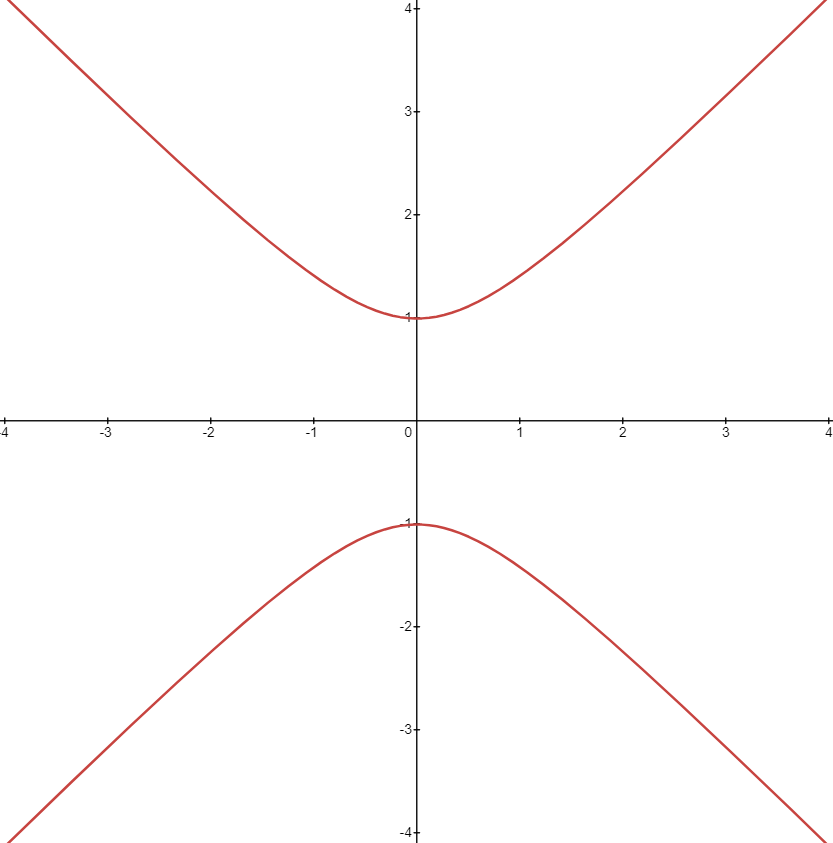
\includegraphics[width=0.5\linewidth]{picture/hyperbola=1.png}
    \caption{Hyperbola of invariant spacetime interval}
    \label{fig:hyperbolic spacetime}
\end{figure}
This means that if we connect a line from the origin to any point on this hyperbola, we should have an invariant spacetime interval. This is the hyperbola of invariant spacetime interval. We can have a series of hyperbola that represents different event and different spacetime intervals. With this graph, it would be easier to find the relationships between events. 


\section{Regions of Spacetime Diagram}
placeholder

\subsection{Speed of Causal Relationship}
There is a speed limit as to how fast causality is, and that is the speed of light. On the spacetime diagram, the region where one can have causal relation with is the region bounded by the 2 diagonal line that represents the speed of light. 

\subsection{Timelike, Spacelike, and Lightlike Events}
In Euclidean Geometry, distance is the sum of 2 squares, therefore it can never be negative.
\[
x^2 + y^2 = r^2
\]
But for spacetime interval, the result could be either positive, negative, or zero depending on which parameter predominates the interaction.
\[
\Delta s^2 = -\Delta t^2 + \Delta r^2
\]
Let's think of some examples to understand the difference. Let there be a train that is traveling with respect to observer in a lab frame. A spark plug flashes twice with a time separation of $\Delta t'$. For observers on the train, 2 flashes or 2 events happened on the same location, hence the spatial separation is zero. Therefore:
\[
-\Delta t'^2 = \Delta s^2 =  -\Delta t^2 + \Delta r^2
\]
We see that we yield a negative number for the spacetime interval. We call this \textbf{Timelike Interval}, and the worldline connecting these 2 events are called \textbf{Timelike Worldline}. And when we have a timelike interval, we would call it the \textbf{Proper Time}\\
\newline
Similarly, we can define another similar situation. The train now has 2 spark plugs with spatial separation $\Delta r'$. For the train, 2 spark plugs would flash simultaneously, meaning that the time separation is zero for the train observer. We have the following relationship:
\[
\Delta r'^2 = \Delta s^2 = -\Delta t^2 + \Delta r^2
\]
We see that the spatial separation predominates the relationship and yielding a positive spacetime interval. We call this a \textbf{Spacelike Interval}. And just like the timelike interval, we would call this spacelike interval the \textbf{Proper Distance}.\\
\newline
One thing to notice is that no worldline can connect 2 events connected by a spacelike interval. This means that 2 events connected by a spacelike interval has no causal relationship, and the sequence of which event happens first can be frame dependent as it would not violate causality.\\
\newline
Lastly, we have a special case. If the 2 events lie on the line that represents the speed of light, or when $\Delta t = \Delta r$, we will have a spacetime interval that is zero.
\[
\Delta s = 0
\]
We call this a \textbf{Lightlike Interval}, since the events are located on the line that is the speed of light. Only particles that can travel at the speed of light, or influence that and propagate at the speed of light can connect 2 events tied by a lightlike interval, such as photon, and gravity. \\
\newline 
We can look at this sample diagram and intuitively understand what are the kinds of intervals. \\

\begin{itemize}
    \item Event 1 $\iff$ Event 3: Timelike Interval/Worldline, Proper time
    \item Event 1 $\iff$ Event 4: Lightlike Interval, Null Interval
    \item Event 1 $\iff$ Event 2: Spacelike Interval, proper distance 
\end{itemize}

\begin{figure}[!h]
    \centering
    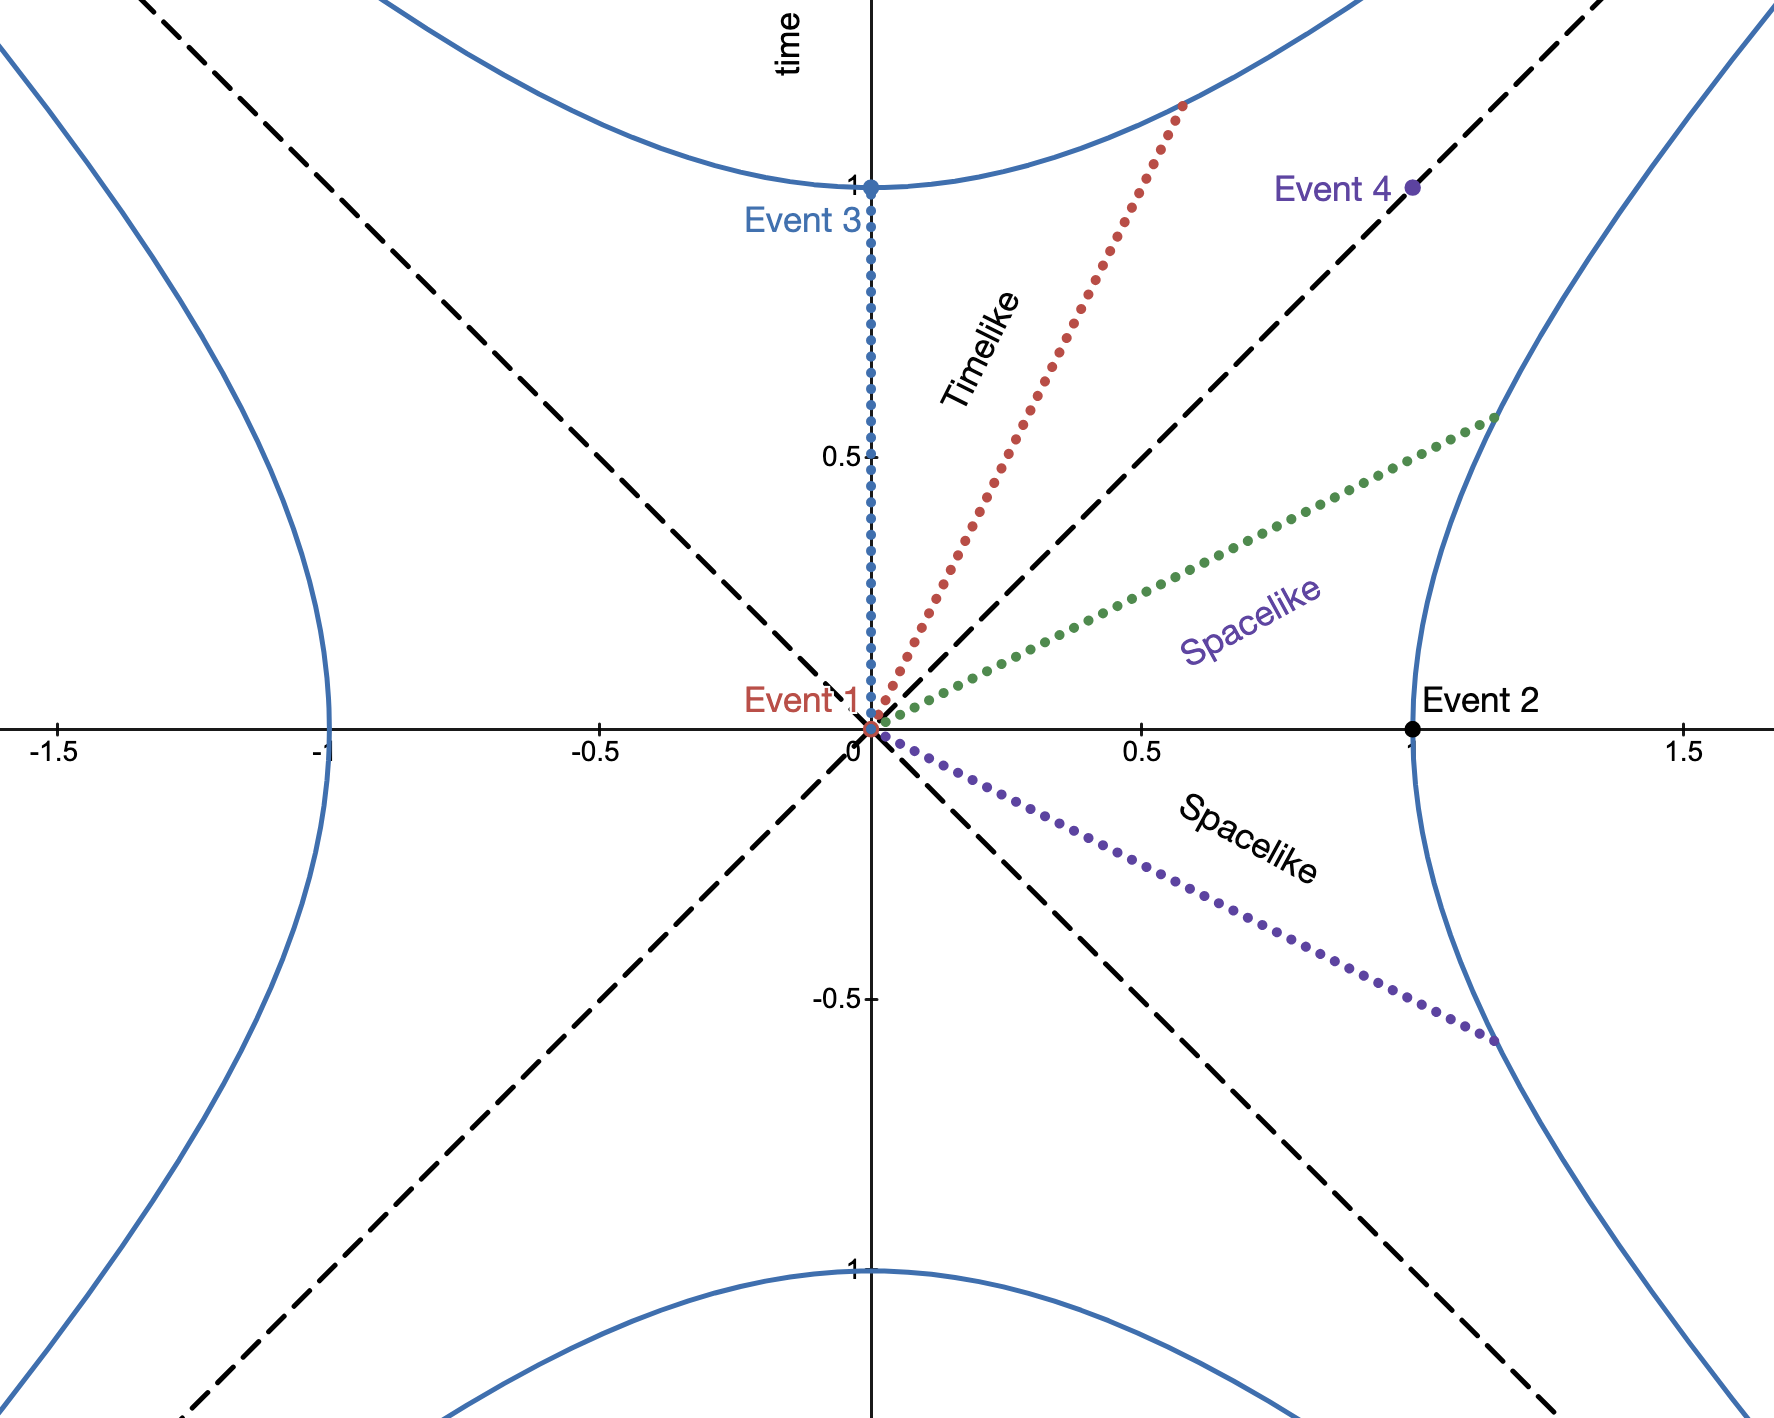
\includegraphics[width=0.5\linewidth]{picture/Spacetime diagram .png}
    \caption{Sample Diagram of different spacetime intervals}
    \label{fig:spacetime diagram}
\end{figure}

\newpage 

\subsection{Light Cone}
Since causality influence our universe at the speed of light, we can think of the speed of light and the distance it travels as the boundary of our interaction, outside which we will never be able to apply any effect. With this in mind, we can dissect our spacetime diagram into 5 different component. \\
\newline
Let us imagine we are at the origin of this spacetime diagram.
\begin{enumerate}
    \item The area shaded blue will be our \textbf{future light cone}, it contains everything that one at the origin will ever be able to alter
    \item The area shaded green is the \textbf{past light cone}, it is all the event that can have a causal relation to us.
    \item The violet boundary of the future light cone is the \textbf{future lightlike region}, where influence would have to propagate at the speed to light to alter anything on this line. Think about \textit{lightlike interval} or \textit{null interval}
    \item The red boundary of the past light cone is similar in nature to the lightlike region of the future light cone, but belongs to the past.
    \item Everything else that is not shaded is the \textbf{spacelike region}, inside which we would never be able to alter, not can it have a causal relation to us. 
\end{enumerate}

\begin{figure}[!h]
    \centering
    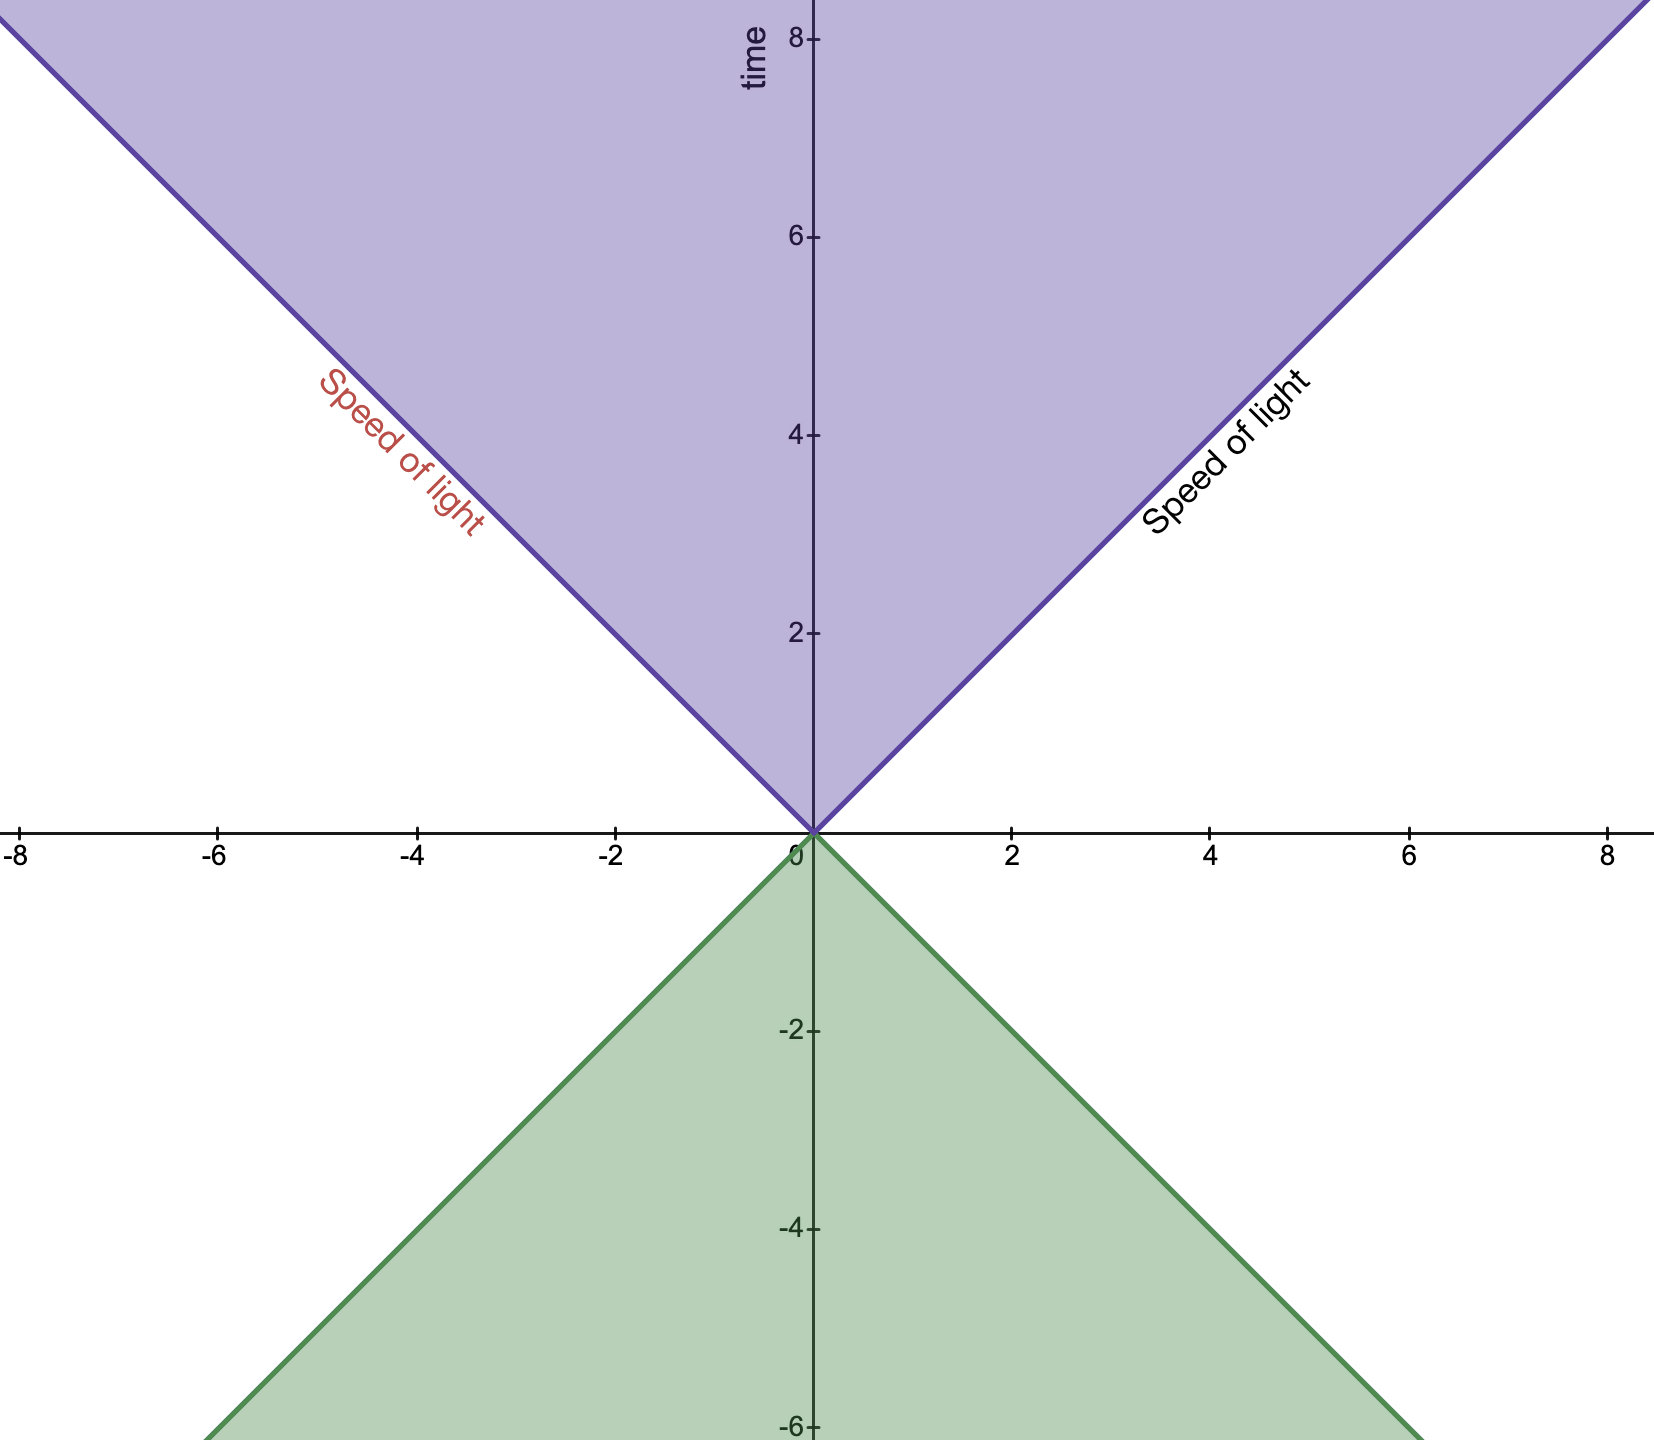
\includegraphics[width=0.5\linewidth]{picture/Light Cone.png}
    \caption{Light Cone}
    \label{fig:lightcone}
\end{figure}

\newpage

\section{Momentum-Energy Conservation}
In this chapter we would seek to treat Momentum and Energy as one group. Conservation of Momentum and Conservation of Energy, or the Newtonian way to understanding motion, fails to work when stuff is happening in relativistic speed. We therefore seek a new way to explore the conservation. We define a term \textbf{Momenergy}, or \textbf{Momentum-energy} to denote this new property.
\subsection{Relationship of Momentum and Energy}
Notice that our notation of speed $\beta$ does not involve a unit. If we consider the classical definition of momentum and energy, $\textbf{p}=m\textbf{v}$ and $E = \frac{1}{2}mv^2$, we would have momentum and energy in the same unit. \\
\newline
We should realize that momenergy is a directed quantity, or a vector, with \textbf{4 components}. It has \textbf{3 dimensions of space} that corresponds with momentum and \textbf{1 dimension of time} for energy. The direction at which the momenergy point is the directed along the worldline between 2 events.\\
\newline
Remember that there is no preferred direction for momenergy. It points at where our test particle is moving, or along the worldline. Let us denote the movement of the particle along the 4-dimensional spacetime with \textbf{spacetime displacement}. This displacement is a vector with 4 components, 1 in time and 3 in space. \\
\newline
Since the momenergy points along the worldline, its direction should be consistent for all inertial frame. And the time we would use for our spacetime displacement would the proper time along the worldline, as that is agreed upon by all inertial frame.\\
\newline
If we were to examine the spacetime diagram, we can figure out the relationship that is somewhat Pythagorean.\\

\begin{figure}[!h]
    \centering
    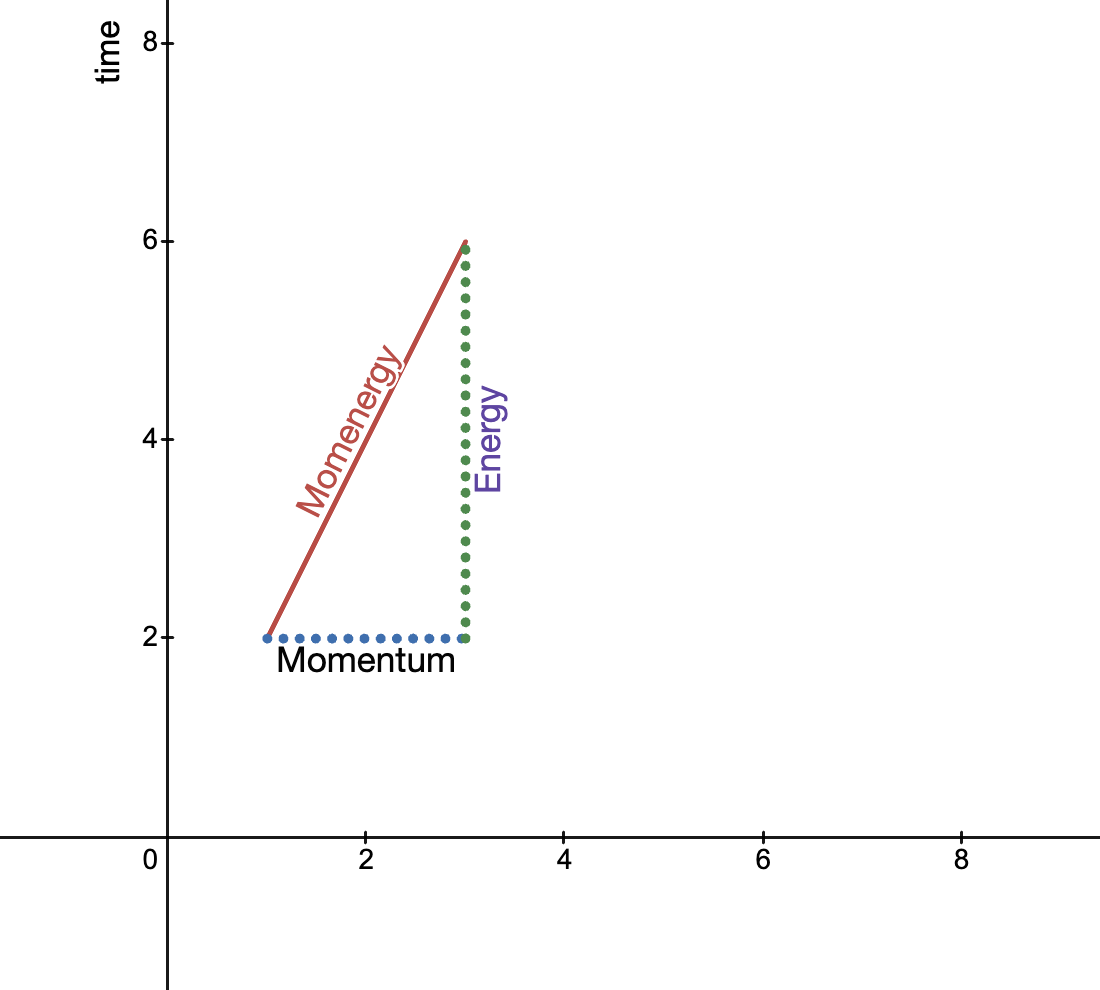
\includegraphics[width=0.5\linewidth]{picture/momentum-energy.png}
    \caption{Relationship Between Momentum and Energy}
    \label{fig:enter-label}
\end{figure}
\newpage
We can derive the following relationship. 
\[
\textbf{Momenergy} = \paren{mass}\times \frac{\paren{\text{spacetime displacement}}}{\paren{\text{proper time of displacement}}}
\]
Our claim is that this momenergy would be conserved between, say, a collision. And before going to the final result, we have revisit what we have concluded so far.
\begin{enumerate}
    \item \textbf{\textit{m} units of mass pursuing a given motion carry \textit{m} times the momenergy of 1 unit of mass.} Momentum is proportional to mass.
    \item \textbf{Momenergy points in the same direction as worldline}.
    \item \textbf{Two event define a worldline between them}, think of it like how 2 points define a line segment.
    \item \textbf{Momenergy is independent of reference frame}, since spacetime interval is independent and agreed upon by all reference frame.
    \item \textbf{We define the direction and magnitude of momenergy 4-vector by 4 unit vectors,} 1 in time, 3 in space. 
    \item \textbf{The momenergy vector is defined as}
    \[
\textbf{Momenergy} = \paren{mass}\times \frac{\paren{\textbf{spacetime displacement}}}{\paren{\text{proper time of displacement}}}
\]
\end{enumerate}

\subsection{Space component of momenergy, Momentum}
We have to be careful here since the numerator of this expression is actually a vector with 4 components $\tribkt{t,x,y,z}$, and is divided by a scalar \textit{proper time}.\\
\newline
We can therefore investigate momenergy of different dimension separately. Let us define proper time to be $\tau$, and $E$ be energy
s
Remember that the momenergy lies on the spacetime interval, our claim is that it has the same magnitude as the spacetime displacement. And since the magnitude of the spacetime displacement should equal to the proper time, we can see that the magnitude of momenergy is simply $\textit{m}$.
\\
\newline
We would also notice that energy and momentum is not conserved across different reference frame, but mass, or momenergy, is. Similar to what we have discussed in the invariant of spacetime interval, an object can have infinite possible momentum and energy as measured in different frames, but its spacetime interval, or mass is agreed upon by all observers. \\
\newline
Why have we not yet noticed the inconsistency of Newtonian mechanics? To answer this question, we can examine the Newtonian expression of momentum. 
\[
\textbf{p}_{Newton} = m\dydx{\textbf{r}}{t}
\]
We notice that the only difference here is the use of $dt$ instead of the proper time $d\tau$. this difference is negligible and hard to detect unless the object is moving in relativistic speed. We know that 
\[
dt = \gamma d\tau
\]
Therefore 
\[
E = m \dydx{t}{\tau} = \gamma m
\]
\[
\textbf{p}_r = m\dydx{\textbf{r}}{\tau} = \gamma m\textbf{v}_r
\]
We see that the difference does not occur until the particle moves with about $\beta=0.3$. For a high energy cosmic ray that shoots through Milky Way, it crosses the entire Milky Way in $30s$ in his own frame while $3\times 10^{12}$ has passed for Earth. The difference gets quite absurd at this speed. 

\subsection{Time component of Momenergy, Energy}
Let's investigate the time component of our 4-vector momenergy, how different is it from our classical definition?\\
\newline 
We have established previously that 
\[
E =m \dydx{t}{\tau} =\gamma m
\]
As before, we consider the classical, or Newtonian definition of kinetic energy:
\[
E_{N} = \frac{1}{2}mv^2
\]
How does this compare to our relativistic definition?
\[
E_{rest} = m
\]
We call $E_{rest}$ the rest energy of the particle. The difference here primarily comes from the fact that, $E_{rest}$ describes the total energy a particle carries, which is a relationship not described in Newtonian mechanics that only describes the \textit{Kinetic Energy} of the Particle. We should make our definition of energy more rigorous. \\
\newline
Let $E$ be our total energy, it should have the following relationship:
\[
E = m + K
\]
Where $m$ is the rest energy and $K$ is the kinetic energy. And from this relationship we can get a relativistic expression for kinetic energy K:
\[
K = E_{tot} - E_{rest} = E - m = m(\gamma - 1)
\]
Now let us look back at \textit{Figure 4}, we notice that the slope of the line of momenergy is simply:
\[
v = \frac{p}{E}
\]
The speed of the particle is the slope of the worldline, therefore the slope of the momenergy. \\
\newline
Now we can get the units sorted out so we can start working on the conversions. Here we will use $E_c$, $K_c$ to denote the converted energy, which should have the same unit across.

\[
E_c = Ec^2 = \gamma mc^2
\]
This is the relativistic total energy of a particle 
\[
E_c = mc^2
\]
This is the rest energy of a particle
\[
K_c = \frac{1}{2}m\beta^2= \frac{1}{2}mv^2c^2 
\]
Here, we get to see the most famous equation of physics in its full glory. $E = mc^2$ demonstrates an incredibly large energy for any mass. But remember that Energy is not the same as mass. We must always remember that it is the rest energy $E_{rest} = mc^2$. Mass is the magnitude of the 4-vector momenergy. 
\subsection{Conservation of Momentum-Energy}
After sorting out our relativistic mechanics, we have come to a very important property that can help us study stuff happening at high speed. \textbf{The conservation of total energy.}\\
\newline
We must realize the potency of this relativistic expression of energy. It includes all sort of energies that is being converted, or transformed in the system during the event. All the interaction of energy is zipped into this \textit{proper time interval}. In the other hand, Newtonian energy is only conserved in perfectly elastic collision, as energy would be converted into heat, sound, and other sort that makes the equivalence invalid. Relativistic mechanics governs \textit{all} interaction of energy. \\
\newline
So how does this conservation translate into calculation and experimental measures?\\
\newline 
Imagine 2 particle collides, and we plot their interaction on the spacetime diagram. The only thing we need to bear in mind is that the sum of the spacetime displacement, or momenergy should add up to a constant that maintain its value before and after the collision. \\
\newpage


Not only that, since we are interested in \textit{the time part of momenergy}, or \textit{energy}, it is also conserved before and after the collision, as we can see from \textit{figure 1.5}. We call this the \textbf{conservation of the time part of momenergy}.
\begin{figure}[t]
    \centering
    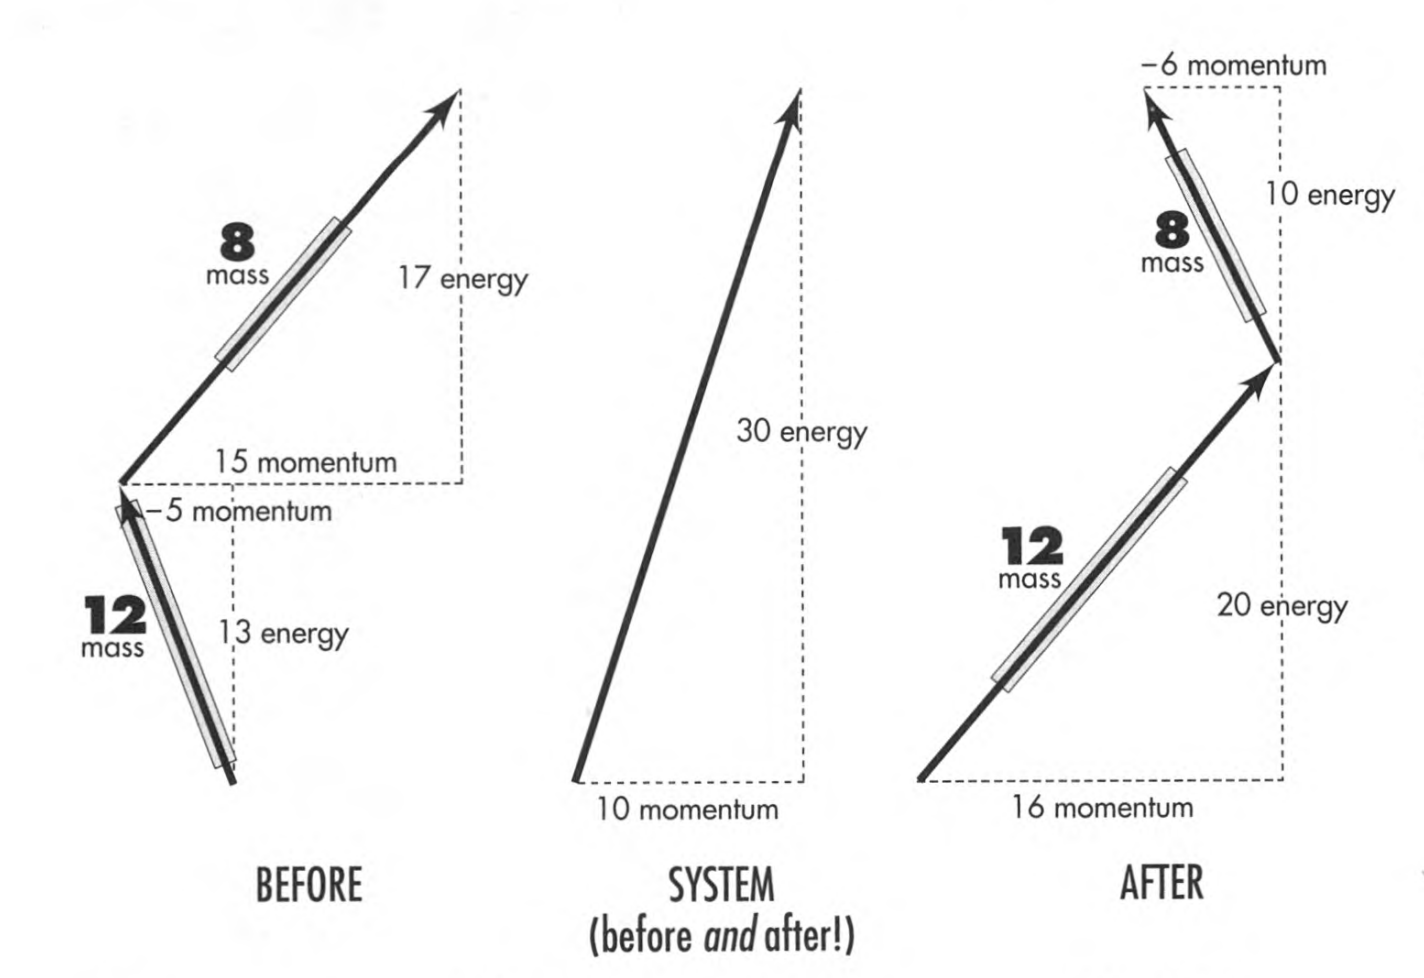
\includegraphics[width=0.5\linewidth]{picture/Momenergy of a system of particles.png}
    \caption{Momenergy of a system of particles (pg 207)}
    \label{fig:pg207}
\end{figure}\\
\newline
What about the space part of the momenergy, the momentum? As we can see from the figure above, it also stays the same before and after the collision, as measured by any inertial frame. Therefore we call this \textbf{Conservation of space part of momenergy}.
\newline
Here, we have a good opportunity to clarity the differences between \textit{invariant}, \textit{conserved}, and \textit{constant}. 
\begin{itemize}
    \item \textbf{Invariant}: A quantity is said to be invariant if it has the same value when measured by observers from reference frames in relative motion with each other. Such as the speed of light, or space time interval.
    \item \textbf{Conserved} We call a quantity conserved if before and and after an encounter, or interaction, it stays the same in a set inertial reference frame. Such as momentum and energy. It is not intrinsic to the event itself and is dependent of frame. 
    \item \textbf{Constant} We say something is constant if it is not dependent of time. Saying something is invariant is different from saying something is constant. Saying a quantity is constant means that when the quantity is recorded, it should not change after time goes on. Such as the speed limit of a highway. Observers on the International Space Station would measure a completely different speed limit for highway but that value would stay constant in his frame. 
\end{itemize}
\subsection{Summary}
Some key takeaway for this section are as follows. Let us denote momenergy with $\textbf{E}_{pE}$, and it is a vector with 4 components, 3 from space and 1 from time. 
\[
\textbf{E}_{pE} \in \R ^4 \Rightarrow \tribkt{E,p_x,p_y,p_z}
\]
\[
\textbf{p} = m\dydx{\textbf{r}}{\tau} \;\;\; \textbf{r} = \tribkt{x,y,z}
\]
The magnitude of the momenergy of a particle is the mass of the particle. 
\[
\abso{\textbf{E}_{pE}}^2 = m
\]
And in a set frame, the components of a particle's momenergy is expressed as:
\[
E = m\dydx{t}{\tau} = \gamma m
\]
And when the particle is at rest
\[
E_{rest} = m
\]
\[
p_x = m\dydx{x}{\tau}\;\;\; p_y = m\dydx{y}{\tau}\;\;\; p_z = m\dydx{z}{\tau}
\]
And the magnitude of the momentum can be expressed as
\[
p = \gamma \beta m
\]
The total energy of the system has the following relationship, $K$ here denotes kinetic energy.
\[
E_{tot}=E_{rest} + K
\]
and we can isolate $K$
\[
K = m(\gamma -1)
\]
An important relationship to notice
\[
\beta = \frac{p}{E}
\]
 Momentum $p$ and Energy $E$ should have the same unit.
\newpage
And the laws of conservation needs to be addressed
\begin{enumerate}
    \item \textbf{Total energy, or time part of momenergy, is conserved before and after an interaction in a given frame.}
    \item \textbf{Momentum, or space part of momenergy, is conserved before and after an interaction in a given frame. }
\end{enumerate}
\begin{figure}[!h]
    \centering
    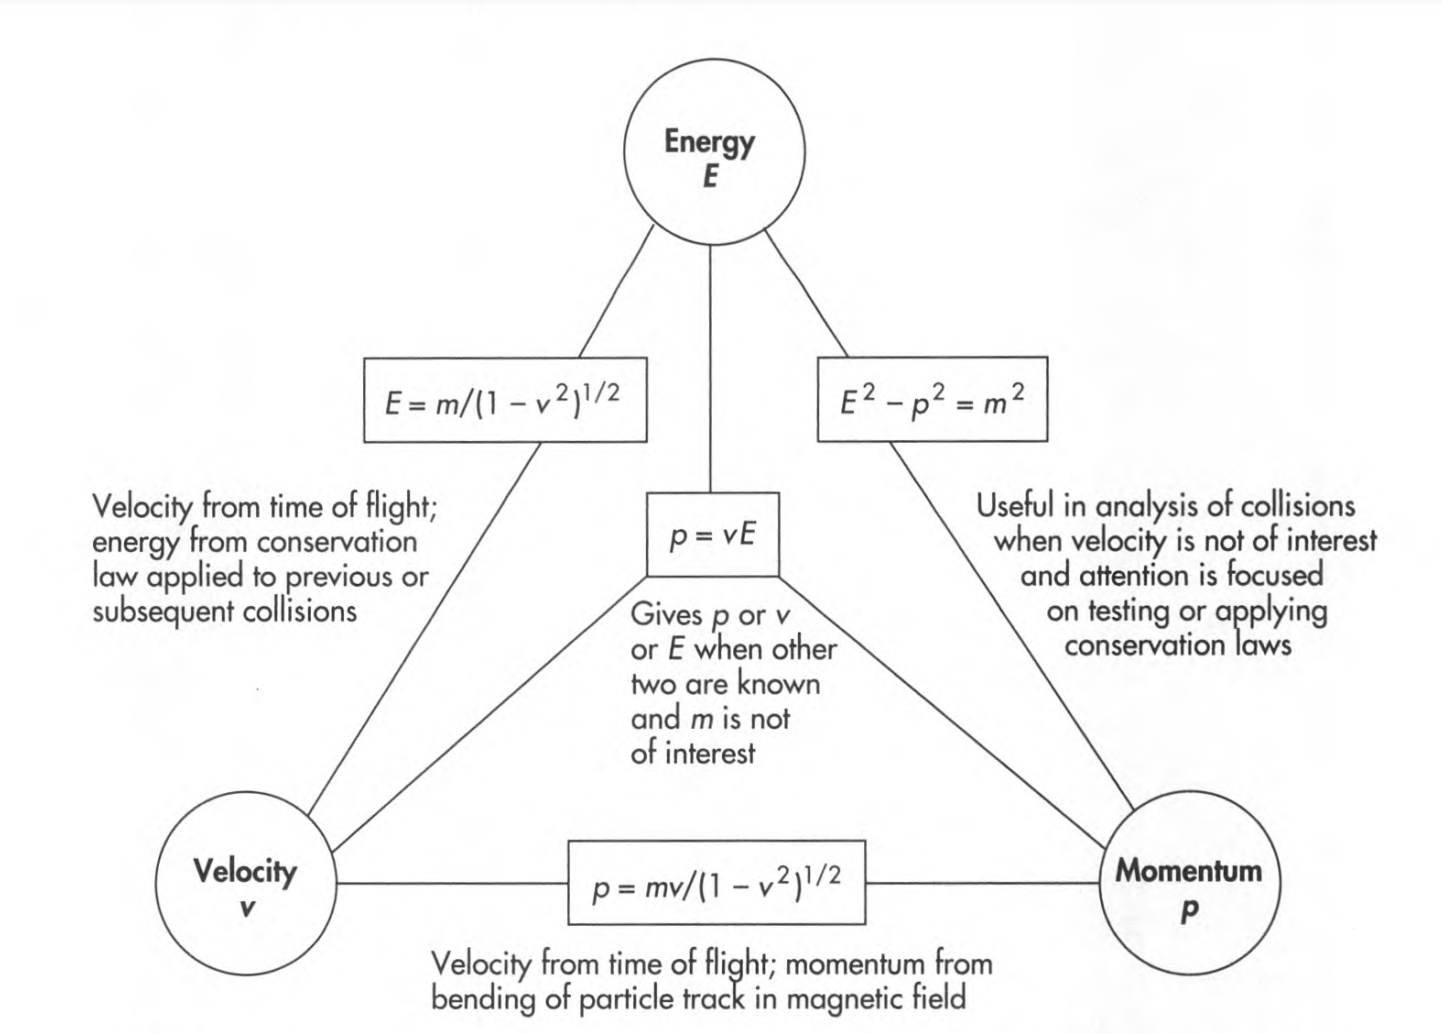
\includegraphics[width=0.5\linewidth]{picture/Momenergy relationship.png}
    \caption{Enter Caption}
    \label{fig:pEconv}
\end{figure}

\subsection{Problems}
\subsubsection{momenergy 4-vector}
For each of the following cases, write down the four components of the momentum-energy 4-vector in the given frame in the form $\tribkt{E,p_x,p_y,p_z}$. Assume that each particle has mass \textit{m}. 
\begin{enumerate}
    \item A particle moves in the positive x-direction in the lab frame with total energy equal to $5E_{rest}$
    \item Same particle as observed in a frame in which it is at rest.
    \item Another particle moves in the z-direction with momentum equal to three times its mass.
    \item Yet another particle moves in the negative y-direction with kinetic energy equal to $4m$.
    \item Still another particle moves with total energy equal to $10m$ and \{$p_x:p_y:p_z = 1:2:3$\}
\end{enumerate}
\textbf{Solutions}
\begin{enumerate}
    \item \(E_{tot}=5m\)
    \[
    K = 25m^2 - m^2 = 24m^2
    \]
    \[
    \textbf{E}_{pE} = \tribkt{5m,2\sqrt{6}\;m,0,0}
    \]
    \item \( E_{tot} = E_{rest} = m\)
    \item \(E_{tot}^2 = E_{rest}^2 + p^2\)
    \[
    E_{tot}^2 = 10m^2
    \]
    \[
    \textbf{E}_{pE} = \tribkt{\sqrt{10}\; m, 0,0,3m}
    \]
    \item \( \textbf{E}_{pE} = \tribkt{3\sqrt{3}\; m},0,-4m,0\)
    \item \(E_{tot} = 10m\)
    \[
    E_{tot}^2 = 100m^2 = \sqbkt{p_x^2+4p_x^2+9p_x^2}+m^2
    \]
    \[
    p_x = \sqrt{\frac{99}{14}}m
    \]
    \[
    \textbf{E}_{pE} = \tribkt{10m,\sqrt{\frac{99}{14}}\;m,2\sqrt{\frac{99}{14}}\;m,3\sqrt{\frac{99}{14}}\;m}
    \]

\end{enumerate}


\section{Relativistic Interactions}
In this section we would explore interactions happened in relativistic context, such as collision, annihilation, or even creation of particle. 

\subsection{System}
We have to define a system on which we would start to do our magic of special relativity.

\subsection{Mass of the System} 
This is a very important concept to grasp in the study of relativity. We are examining \textit{rest mass} of the entire system we are interested in. It is a \textit{property} of the system, and it is an inherent characteristic that cannot be attributed to any specific entity in the system nor does it manifest in a specific form. Asking where the mass of the system is located is a poorly worded problem. Nature demands a conservation of total energy before and after an interaction, therefore we found this quality that satisfy this demand.\\
\newline
We have to realize that, although kinetic energy and momentum has been following a linear relationship, meaning we can add or subtract easily, mass addition does not follow a linear relationship in the system. Now let's do a few examples to make the concept solid. Remember, to study this system, we have to ensure it is an \textbf{isolated system}. As long as the system is isolated, we can choose an arbitraty frame to study it and will get an invariant rest mass for the system.  \\
\subsubsection{Sample Problem I}
Compute $m_{sys}$ for all the following case, assuming all the particle in question are of mass $m$ unless otherwise stated.
\begin{enumerate}
    \item System A: \\
    Particle 1: \(K = 3m \hat{\textbf{x}}\)\\
    Particle 2: \(K = 0\)
    \item System B:\\
    Particle 1: \(K = 5m \hat{\textbf{x}}\)\\
    Particle 2: \(K = 5m \hat{\textbf{x}}\)
    \item System C:\\
    Particle 1: \(E_{rest} = 3m\), \(\textbf{E} = 7m \hat{\textbf{x}}\)\\
    Particle 2: \(K = 0m \hat{\textbf{x}}\)
    \item System D:\\
    Particle 1: \(\textbf{E}=-6m\hat{\textbf{y}}\)\\
    Particle 2: \(\textbf{E}=6m\hat{\textbf{x}}\)
\end{enumerate}
\subsubsection{Solution I}
\begin{enumerate}
    \item System A:
    \[
    E_1 = 3m + m = 4m\]
    \[
    p_1 = \sqrt{15}m = p_{sys}
    \]
    \[
    E_{sys} = 3m + 2m = 5m
    \]
    \[
    m_{sys} = \sqrt{E_{sys}^2-p_{sys}^2}=\sqrt{10}m
    \]
    \item System B:\\
    Particles 1 and 2 are not in relative motion. Therefore the mass of the system is simply $m_{sys} = 2m$. Mathematical proof:
    \[
    E_1 = E_2 = 6m
    \]
    \[
    E_{tot}=12m
    \]
    \[
    p_1 = p_2 = \sqrt{35}m
    \]
    \[
    p_{tot}=2\sqrt{35}m
    \]
    \[
    m_{sys} = \sqrt{144 - 140} = 2m
    \]
    \item 
\end{enumerate}

\subsection{Energy and Mass}
Energy can be transferred with mass-less medium such as photon. A photon carries only momentum but not kinetic energy. And it has a wave length of 
\[
\lambda = \frac{h}{p}
\]
$h$ here is the plank constant. Also, since a photon is mass-less, it means that its momenergy points in the lightlike direction, and its motion traces the lightlike worldline. And since it has no kinetic energy, its energy can be easily expressed as 
\[
E = p 
\]
Here, p represents the momentum of the photon, and E is the energy that proton carries. \\
\newline

We get to see the effect of a photon interaction when a photon scatters off an election. Compton first discovered this effect and derived a theory that quantize the energy of light, which was a monumental event in the study of quantum physics.\\
\newline
With enough energy, mass can even be conjured out of nowhere. A photon carrying $p=4m_e$ can hit an electron at rest and create a pair of $e^-$ and $e^+$, an electron and a positron. These particles would form a structure called $polyelectron$ which will keep moving in the direction of the original photon. And the photon that caused the incident would scatter and turn around going to opposite direction. This is called a \textbf{backward scattering}. \\
\newline
If you would accelerate something heavier like a proton and clash it with another proton, you can make heavier particles out of nowhere. And when a pair of matter and antimatter, such as electron and position, touches each other, they would annihilate and convert all its mass to energy. This is probably the most efficient way of obtaining energy. Way more efficient than nuclear fission and fusion which also harvest the conversion of mass to energy. \\
\newline
Do keep in mind that energy and mass are not always convertible, and they have to comply with the 2 fundamental laws in relativity:
\begin{itemize}
    \item \textbf{Invariant of Momenergy of isolated system, and conservation of Momenergy before and after interactions in an isolated system.}
    \item \textbf{The invariant magnitude of the momenergy of a particle equals the rest mass of that particle. }
\end{itemize}

\subsection{Wrapping up: Questions to think about}
This section will wrap up our study so far nicely. It will be consisted of questions and answers to some interesting topics. 
\begin{enumerate}

    \item Does an isolated system have the same mass as observed in every inertial (free-float) reference frame?
    \item[Answer:] Yes, think of rest mass as the spacetime interval, where the space interval is momentum and time interval is energy. The mass should be invariant across reference frame just like spacetime interval.
    \item Does its energy have the same value in every inertial frame?
    \item[Answer:]No, momentum and energy can vary in different reference frame. 
    \item Does energy equal zero for an object of zero mass, such as a photon?
    \item[Answer:]No, Photons obviously have energy as discussed previously. Its energy equals its momentum. 
    \item Can a photon — that has no mass— give mass to an absorber?
    \item[Answer:] This is certainly possible, such as the example of the positron electron pair created by the photon. Mass was created. 
    \item Invariance of mass; Is that feature of nature the same as the principle that all electrons in the universe have the same mass?
    \item[Answer:] The invariance of mass is describing a more general case than the elementary particles. It says that for any reference frame, even if the observation for kinetic energy and momentum is different, everyone should come to the same conclusion as to what the rest mass it.
    \item Momenergy: Is that a richer concept than mass?
    \item[Answer:] Yes it is. It describes the direction of the particle in the spacetime diagram rather than being a scalar that provides no additional information. 
\end{enumerate}

\subsection{Problems}
WIP

\chapter{Intro to Electrodynamics - Griffiths}
\section{Electrodynamics and Relativity (12.1)}
\subsection{\textbf{12.1 The Special Theory of Relativity}}
\subsubsection{\textbf{12.1.1 Einstein’s Postulates}}
        \begin{enumerate}
            \item \textbf{The principle of relativity.} The laws of physics apply in all inertial reference systems.
            \item \textbf{The universal speed of light.} The speed of light in vacuum is the same for all inertial observers, regardless of the motion of the source.
        \end{enumerate}
\newline Although it developed historically out of Einstein’s contemplation
of electrodynamics, the special theory is not limited to any particular class
of phenomena—rather, it is a description of the space-time “arena” in which all
physical phenomena take place. And in spite of the reference to the speed of light
in the second postulate, relativity has nothing to do with light: c is a fundamental
velocity, and it happens that light travels at that speed, but it is perfectly possible
to conceive of a universe in which there are no electric charges, and hence
no electromagnetic fields or waves, and yet relativity would still prevail.
\subsubsection{\textbf{12.1.2 The Geometry of Relativity}}
    \begin{enumerate}
        \item \textbf{The relativity of simultaneity}: Two events that are simultaneous in one inertial system are not, in general, simultaneous in another. An \textbf{observation} is an artificial reconstruction after the fact, when all the data are in, and it doesn’t depend on where the observer is located. In fact, a wise observer will avoid the whole problem by stationing assistants at strategic locations, each equipped with a watch synchronized to a master clock, so that time measurements can be made right at the scene.
        \item \textbf{Time dilation}: Moving clocks run slow. $\bar{\Delta t} = \sqrt{1 - \frac{v^2}{c^2}}\Delta t$. Evidently, the time elapsed between the same two events (light leaves bulb, and light strikes center of floor) is different for two observers (inside the train and outside). In fact, the interval recorded on the train clock, $\bar{t}$, is shorter by the factor $\gamma \equiv \frac{1}{\sqrt{1 - \frac{v^2}{c^2}}}$. 
        Because moving clocks are not synchronized, it is essential when checking time dilation to focus attention on a single moving clock. All moving clocks runs low by the same factor, but you can’t start timing on one clock and then switch to another because they weren’t in step to begin with. But you can use as many stationary clocks (stationary with respect to you, the observer) as you please, for
        they are properly synchronized (moving observers would dispute this, but that’s their problem).
        \item \textbf{Lorentz contraction}: Moving objects are shortened. Dimensions perpendicular to the velocity are not contracted. $\bar{x} = x \sqrt{1 - \frac{v^2}{c^2}}$.
    \end{enumerate}
\subsubsection{\textbf{12.1.3 The Lorentz Transformations}}
Suppose we know the coordinates $(x, y, z, t)$ of a particular event $E$ in one inertial system $S$, and we would like to calculate the coordinates $(\bar{x}, \bar{y}, \bar{z}, \bar{t})$ of that same event in some other inertial system $\bar{S}$. What we need is a “dictionary” for translating from the language of $S$ to the language of $\bar{S}$. We may as well orient our axes, so that $\bar{S}$ slides along the $x$ axis at speed $v$. If we “start the clock” $(t = 0)$ at the moment the origins $(O $ and $ \bar{O})$ coincide, then at time $t$, $\bar{O}$ will be a distance $vt$ from $O$, hence the Lorentz Transformations:

\begin{enumerate}
    \item $\bar{x} = \gamma (x - vt)$
    \item $\bar{y} = y$
    \item $\bar{z} = z$
    \item $\bar{t} = \gamma \left( t - \frac{v}{c^2} x \right)$
\end{enumerate}

\textbf{Rules for Translating Angles:} There is no universal rule for translating angles — you have to know whether it’s an angle made by a velocity vector $\mathbf{\tan{\theta}=\frac{u_y}{u_x}=\frac{1}{\gamma}\frac{\bar{u}_y}{\bar{u}_x+v}}$ or a position vector $\mathbf{\tan{\theta}=\gamma\frac{\sin{\bar{\theta}}}{\cos{\bar{\theta}}}}$.]

\subsection{\textbf{12.1.4 The Structure of Spacetime}}
\begin{enumerate}
    \item \textbf{Four-vectors.} The Lorentz transformations take on a simpler appearance when expressed in matrix form (where $x^0=ct, \beta = \frac{v}{c}, x^1=x, x^2=y, x^3=z$): 
    \[
    \begin{pmatrix}
    \bar{x}^0 \\
    \bar{x}^1 \\
    \bar{x}^2 \\
    \bar{x}^3
    \end{pmatrix}
    =
    \begin{pmatrix}
    \gamma & -\gamma\beta & 0 & 0 \\
    -\gamma\beta & \gamma & 0 & 0 \\
    0 & 0 & 1 & 0 \\
    0 & 0 & 0 & 1
    \end{pmatrix}
    \begin{pmatrix}
    x^0 \\
    x^1 \\
    x^2 \\
    x^3
    \end{pmatrix}
    \]   
    Letting Greek indices run from 0 to 3, this can be distilled into a single equation:
    \[
    \bar{x}^\mu = \sum_{\nu=0}^{3} (\Lambda^\mu_{\ \nu}) x^\nu,
    \]
\end{enumerate}
where $\Lambda$ is the \textbf{Lorentz transformation matrix} (the superscript $\mu$ labels the row, the subscript $\nu$ labels the column). \\
The \textbf{four-dimensional scalar product} (is invariant under $\Lambda$ just like ordinary dot product is invarient under rotation): 
\[ 
-a^0b^0+a^1b^1+a^2b^2+a^3b^3 = =a^0b^0 + \mathbf{a \cdot b} 
\]
Introduce \textbf{covariant} vector $a_{\mu}$ , which differs from \textbf{contravariant}  $a^{\mu}$ only in the sign of zeroth component:
\[
a_{\mu}=(a_0, a_1, a_2, a_3)=(-a^0, a^1, a^2, a^3)
\] Note, that raising or lowering a temporal index costs a minus sign $(a_0=-a^0)$.  Formally the \textbf{Minkowski metric}, 
\[
a_{\mu} = \sum_{\nu=0}^{3} g_{\mu\nu} a^\nu , \quad \text{where} \quad g_{\mu\nu} \equiv
\begin{pmatrix}
-1 & 0 & 0 & 0 \\
0 & 1 & 0 & 0 \\
0 & 0 & 1 & 0 \\
0 & 0 & 0 & 1
\end{pmatrix}
\]
The scalar product can now be written with summation symbol,
\[
\sum_{\mu=0}^{3} a^{\mu} b_\mu \quad \text{ or, more compactly, } \quad a^\mu b_\mu =a_\mu b^\mu
\]
This is called the \textbf{Einstein summation convention}.
\section{12.2}
placeholder
\section{12.3}
placeholder

\chapter{Intro to Elementary Particles - Griffiths}
\section{Relativistic Kinematics (Chapter 3)}
placeholder

\chapter{A First Course in GR - Schultz}
WIP
\section{Chapter 1}
WIP
\section{Chapter 2}
WIP
\section{Chapter 3}
WIP
\section{Chaoter 4}
WIP

















\end{document}
